\documentclass[modern, letterpaper]{aastex62}
% \documentclass[twocolumn, letterpaper]{aastex62}

\include{gitstuff}
% Load common packages
% \usepackage{microtype}  % ALWAYS!
\usepackage{amsmath}
\usepackage{amsfonts}
\usepackage{amssymb}
\usepackage{booktabs}

\usepackage{graphicx}
\usepackage{color}

\definecolor{cbblue}{HTML}{3182bd}
\usepackage{hyperref}
\definecolor{linkcolor}{rgb}{0.02,0.35,0.55}
\definecolor{citecolor}{rgb}{0.45,0.45,0.45}
\hypersetup{colorlinks=true,linkcolor=linkcolor,citecolor=citecolor,
            filecolor=linkcolor,urlcolor=linkcolor}
\hypersetup{pageanchor=true}

\newcommand{\documentname}{\textsl{Article}}
\newcommand{\sectionname}{Section}
\renewcommand{\figurename}{Figure}
\newcommand{\eqname}{Equation}
\renewcommand{\tablename}{Table}

% Packages / projects / programming
\newcommand{\package}[1]{\textsl{#1}}
\newcommand{\acronym}[1]{{\small{#1}}}
\newcommand{\github}{\package{GitHub}}
\newcommand{\python}{\package{Python}}
\newcommand{\emcee}{\project{emcee}}

% Missions
\newcommand{\project}[1]{\textsl{#1}}

% For referee
\newcommand{\changes}[1]{{\color{red} #1}}

% Stats / probability
\newcommand{\given}{\,|\,}
\newcommand{\norm}{\mathcal{N}}

% Maths
\newcommand{\dd}{\mathrm{d}}
\newcommand{\transpose}[1]{{#1}^{\mathsf{T}}}
\newcommand{\inverse}[1]{{#1}^{-1}}
\newcommand{\argmin}{\operatornamewithlimits{argmin}}
\newcommand{\mean}[1]{\left< #1 \right>}

% Unit shortcuts
\newcommand{\msun}{\ensuremath{\mathrm{M}_\odot}}
\newcommand{\kms}{\ensuremath{\mathrm{km}~\mathrm{s}^{-1}}}
\newcommand{\mps}{\ensuremath{\mathrm{m}~\mathrm{s}^{-1}}}
\newcommand{\pc}{\ensuremath{\mathrm{pc}}}
\newcommand{\kpc}{\ensuremath{\mathrm{kpc}}}
\newcommand{\kmskpc}{\ensuremath{\mathrm{km}~\mathrm{s}^{-1}~\mathrm{kpc}^{-1}}}

% Misc.
\newcommand{\bs}[1]{\boldsymbol{#1}}
\definecolor{mahogany}{RGB}{165,15,21}
\newcommand{\resp}[1]{{\color{mahogany}#1}}

% Astronomy
\newcommand{\DM}{{\rm DM}}
\newcommand{\feh}{\ensuremath{{[{\rm Fe}/{\rm H}]}}}
\newcommand{\df}{\acronym{DF}}

% TO DO
\newcommand{\todo}[1]{{\color{red} TODO: #1}}


% adjust AAS-TEX shit
% \setlength{\parindent}{1.1\baselineskip}

\graphicspath{{figures/}}

% define macros for text
\newcommand{\apogee}{\project{\acronym{APOGEE}}}
\newcommand{\sdssiv}{\project{\acronym{SDSS-IV}}}
\newcommand{\thejoker}{\project{The~Joker}}
\newcommand{\thecannon}{\project{The~Cannon}}
\newcommand{\DR}{\acronym{DR14}}
\newcommand{\DRtw}{\acronym{DR12}}
\newcommand{\RC}{\acronym{RC}}
\newcommand{\RGB}{\acronym{RGB}}
\newcommand{\quantile}[2]{\ensuremath{\textrm{Q}_{#1}}\left(#2\right)}
\newcommand{\pdf}{\textit{pdf}}
\newcommand{\logg}{\ensuremath{\log g}}
\newcommand{\Teff}{\ensuremath{T_{\textrm{eff}}}}
\newcommand{\med}[1]{\ensuremath{\textrm{med}\left(#1\right)}}
\newcommand{\Psurf}{\ensuremath{P_\textrm{surface}}}

\newcommand{\nunimodal}{320}
\newcommand{\nclean}{234}

% for response to referee
% \renewcommand{\resp}[1]{#1}

\shortauthors{Price-Whelan et al.}

\begin{document}\sloppy\sloppypar\raggedbottom\frenchspacing % trust me

\title{Binary companions of evolved stars in \apogee\ \DR: \\
       Orbital circularization}

\author[0000-0003-0872-7098]{Adrian~M.~Price-Whelan}
\affiliation{Department of Astrophysical Sciences,
             Princeton University, Princeton, NJ 08544, USA}
\email{adrn@astro.princeton.edu}
\correspondingauthor{Adrian M. Price-Whelan}

% \author[0000-0003-2866-9403]{David~W.~Hogg}
% \affiliation{Max-Planck-Institut f\"ur Astronomie,
%              K\"onigstuhl 17, D-69117 Heidelberg, Germany}
% \affiliation{Center for Cosmology and Particle Physics,
%              Department of Physics,
%              New York University, 726 Broadway,
%              New York, NY 10003, USA}
% \affiliation{Center for Data Science,
%              New York University, 60 Fifth Ave,
%              New York, NY 10011, USA}
% \affiliation{Flatiron Institute,
%              Simons Foundation,
%              162 Fifth Avenue,
%              New York, NY 10010, USA}

% \author[0000-0003-4996-9069]{Hans-Walter~Rix}
% \affiliation{Max-Planck-Institut f\"ur Astronomie,
%              K\"onigstuhl 17, D-69117 Heidelberg, Germany}

\begin{abstract}\noindent % trust me
% Context
Short-period binary star systems dissipate orbital energy through tidal
interactions that lead to tighter, more circular orbits.
When at least one star in a binary has evolved off of the main sequence, orbital
circularization occurs for longer-period ($\approx 100~\textrm{day}$) systems.
It has been shown that the orbital parameters and the circularization periods of
a small sample of binary stars with evolved star members can be understood
within the context of standard tidal circularization theory.
% Aims
Using a sample of binaries with subgiant, giant, and red clump star members that
is nearly an order of magnitude larger in size relative to previous work, we
reexamine predictions for tidal circularization of binary stars with evolved
star members.
% Methods
% Results
We confirm that, using equilibrium tide theory, systems predicted to have
circularized generally have negligible measured eccentricities.
We additionally show that the circularization period is correlated with the
surface gravity (i.e. size) of the evolved star member, indicating that the
circularization timescale must be shorter than the evolutionary timescale along
the giant branch.
A few systems are exceptions to the conclusions above and are mentioned in the
discussion.

\end{abstract}

\keywords{
  binaries:~spectroscopic
  --
  binaries:~close
  --
  stars:~evolution
  --
  stars:~interiors
}

\section{Introduction} \label{sec:intro}

From studies of binary star systems in open clusters, it is clear that
short-period binaries tend to have smaller eccentricities as compared to
longer-period binaries of the same age (e.g., \citealt{Mathieu:2005}).
Within a given population of binaries, this manifests as an apparently steep
transition from a spread in eccentricities to mainly circularized orbits
that occurs around some characteristic period (see, e.g., \figurename~5 in
\citealt{Mathieu:2005}) that depends on the age and evolutionary state of the
population.
Many studies have measured the ``circularization period,'' predominantly for
main-sequence binaries (e.g., \citealt{Latham:2002, Meibom:2006,
Kjurkchieva:2017}), and have found that it tends to be between 5--20 days,
depending on age (e.g., \citealt{Mathieu:1988}).
For giant stars, the circularization period appears to be longer, closer to
$\approx 100$ days (e.g., \citealt{Mayor:1984, Bluhm:2016}), but fewer systems
with giant star members have been studied.
These observed trends are likely a result of orbital circularization rather than
a manifestation of binary star formation, as the circularization or transition
period appears to vary with the age of the population (\citealt{Meibom:2005}).

Theories that explain orbital circularization generally rely on tidal
dissipation to explain and predict the timescales of this phenomenon (see
\citealt{Mazeh:2007hp} for a review).
For stars with deep convective zones (and especially evolved stars), the
equilibrium tide theory for circularization (\citealt{Zahn:1977, Zahn:1989}) has
been shown to reasonably reproduce the circularization periods of a small sample
of binaries with giant star members in open clusters (\citealt{Verbunt:1995}).
In this theory, the tidal bulge induced on the primary (evolved) star will lag
the orbital motion of the companion because of coupling of the tidal flow to
turbulent eddies driven by convection.
These eddies cause an effective viscosity in the convective region of the
primary star, and the magnitude of this viscosity affects the amount of lag,
which directly relates to the circularization timescale for a given binary
system (\citealt{Zahn:1989}; also summarized in \citealt{Goodman:1997}).
This viscous dissipation of orbital energy acts to synchronize and circularize a
binary system (\citealt{Zahn:1977, Zahn:1989}).

In the context of equilibrium tide theory, the time-dependence of the
eccentricity, $e$, and semi-major axis, $a$, of a binary star system is given by
\begin{align}
    \frac{1}{t_\textrm{circ}} &= f \,
        \left(\frac{L_1}{M_{\textrm{env}} \, R_1^2}\right)^{1/3} \,
        \frac{M_{\textrm{env}}}{M_1} \,
        q \, (1 + q) \,
        \left(\frac{R_1}{a}\right)^8 \label{eq:tcirc}\\
    \frac{1}{e} \, \frac{\dd e}{\dd t} &= - \frac{1}{t_\textrm{circ}}
        \label{eq:dlne} \\
    \frac{1}{a} \, \frac{\dd a}{\dd t} &= - \frac{38}{7} \, e^2 \,
        \frac{1}{t_\textrm{circ}} \label{eq:dlna}
\end{align}
where $L_1, M_1, R_1$ are the luminosity, mass, and radius of the primary
(evolved) star, $M_{\textrm{env}}$ is the mass of the convective envelope of the
primary, $q = M_2 / M_1$ is the binary mass ratio, $a$ is the binary semi-major
axis, and $f$ is a dimensionless factor of order unity that depends on the
convective and dissipative properties of the convective envelope
(\citealt{Zahn:1977,Zahn:1989,Verbunt:1995}).
Following \citet{Verbunt:1995}, we set $f=1$.

The steep $\left(R_1 / a\right)^8$ scaling in \eqname~\ref{eq:tcirc}
implies that, for a given binary, even small changes in the radius of the
primary results in very large changes to the circularization timescale.
For example, for binary stars with periods $P \gtrsim 10~\textrm{day}$, we
expect orbital circularization to occur rapidly only as the primary begins to
evolve.
Further, if the circularization timescale (\eqname~\ref{eq:tcirc}) remains short
compared to the evolutionary timescale along the subgiant and giant branches,
then the circularization period of a sample of binary stars should correlate
with the radius or evolutionary state of the primary.

Using a significantly larger sample of binary star systems with at least one
evolved member, we study the circularization period along the giant branch.
We show that indeed the inferred circularization period is a function of the
surface gravity of the primary star, and thus that orbital circularization must
occur faster than post-main-sequence stellar radius and structure evolution.

In \sectionname~\ref{sec:data}, we describe the original data source and catalog
of binary star systems used in this work.
In \sectionname~\ref{sec:results}, we show how the circularization period changes in bins of primary-star surface gravity.
In \sectionname~\ref{sec:discussion}, we discuss \todo{...}

% Past work on samples of binary systems with giant star members showed
% that, while main sequence binaries have circularization periods near $\sim
% 10~\textrm{day}$, the circularization period for the giant star binaries is
% typically $\sim 100~\textrm{day}$ (\citealt{Mayor:1984}).
% For a subset of 28 giant star binaries in open clusters (and therefore have age
% estimates), VP95 also show that the systems predicted to be circular (those
% predicted to have large $\Delta \ln e$) do indeed have small measured
% eccentricities.

\section{Data} \label{sec:data}

To identify binaries, we use sources with repeat radial velocity measurements in
data release 14 (\DR) of the \apogee\ survey
(\citealt{Majewski:2017,Abolfathi:2017}), a component of the Sloan Digital Sky
Survey IV (\sdssiv; \citealt{Gunn:2006,Blanton:2017}).
A full description of our search methodology and binary star catalogs can be
found in companion work (\citealt{Price-Whelan:2018}).

Briefly, we use a custom-built Monte Carlo sampler (\package{The Joker};
\citealt{Price-Whelan:2017}) to generate posterior samples over binary orbital
parameters (period, eccentricity, etc.) for all stars with $\geq 3$ radial
velocity measurements in \apogee\ \DR\ that pass a series of quality cuts.
By making cuts on our posterior belief about the amplitude of radial velocity
variations, we identified $\sim$5,000 binary star systems with at least one
evolved star member.
However, the majority of these systems have too few radial velocity measurements
to uniquely determine the binary orbital parameters.

Here, we only consider \nunimodal\ binary systems for which the period and
eccentricity can be uniquely determined (the ``high-$K$, unimodal'' sample of
\citealt{Price-Whelan:2018}).
We further subselect the \nclean\ primary stars with $\logg > 2$ and that pass
visual inspection (from previous work, \texttt{clean\_flag == 0}; see
\sectionname~5.2 in \citealt{Price-Whelan:2018}).
\figurename~\ref{fig:logg-teff-m1} (left) shows the stellar parameters for all
\nclean\ primary stars in the sample used in this work.
\figurename~\ref{fig:logg-teff-m1} (right) shows the distribution of primary
masses for the 68 systems with masses from \cite{Ness:2015}.

% Notebook: Period-eccentricity
\begin{figure}[h]
\begin{center}
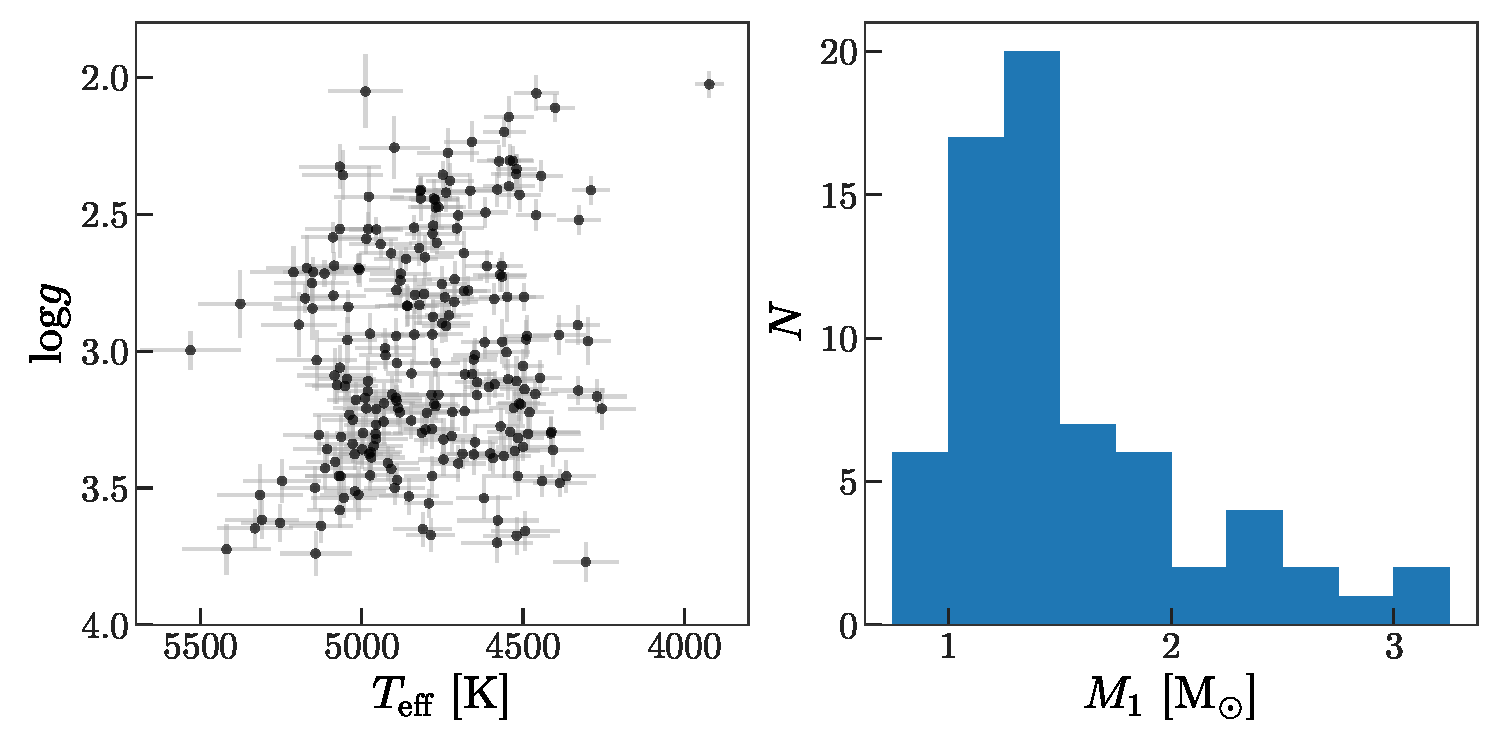
\includegraphics[width=\textwidth]{logg-teff-m1}
\end{center}
\caption{%
\textit{Left}: Stellar parameters for all \nclean\ systems used in this work.
Effective temperatures, \Teff, and surface gravities, \logg, are from the
\apogee\ \DR\ catalog.
\textit{Right}: Primary masses for 68 systems used in this work with masses
estimated in cite{Ness:2015}.
\label{fig:logg-teff-m1}
}
\end{figure}


\section{Population synthesis}
\label{sec:theory}

To compare with the data, we generate a simulated population of binary star
systems with primary stars that have similar stellar parameters (by the end of
their evolution) to our sample of \apogee\ system primaries.
We assume simple initial binary orbital parameter distributions (i.e. in period
and eccentricity) and compute the change in eccentricity and separation of the
companion orbit as the primary star evolves off the main sequence.

In detail, we sample primary stellar masses, companion masses, and primary
surface gravities by fitting two-component Gaussian mixture models (GMMs) to the
stars in our sample with measurements of each, then re-sample using the fitted
distributions.
As described in previous work (\citealt{Price-Whelan:2018}), primary mass
measurements come from \cite{Ness:2015}, secondary (minimum) masses come from
the posterior samplings over orbital parameters using \apogee\ radial velocity
data, and surface gravities come from the \apogee\ (\DR) data reduction pipeline
(\citealt{Garcia-Perez:2016}).
In our sample, the median primary mass, companion mass, and surface gravity are
$\med{M_1} = 1.4~\msun$, $\med{M_{2, \textrm{min}}} = 0.4~\msun$, and
$\med{\logg} = 3.1$.
We assume $M_2 = M_{2, \textrm{min}}$ when generating companion masses.

We generate eccentricities $e$ by sampling from a beta distribution with
parameters $(a, b) = (1, 2)$, meant to mimic the distribution of eccentricities
for long-period binary systems in our sample.
We generate initial binary orbital periods, $P$, by assuming a distribution that
is uniform in $\ln P$ between $(\Psurf, 8192)~\textrm{day}$, where
\Psurf\ is the orbital period at which the minimum separation is
equal to the surface size of the primary star,
\begin{align}
    \Psurf &= 2\pi \,
        \left(\frac{G \, (M_1+M_2)}{R_1^3}\right)^{-1/2} \,
        \left(1-e\right)^{-3/2}
    \quad . \label{eq:Psurf}
\end{align}
\figurename~\ref{fig:simulated} (left) shows the initial periods and
eccentricities of the simulated systems.
Markers are colored by the mass of the primary, $M_1$, and the size of the
marker indicates the log-surface gravity, \logg.

To follow the stellar evolution of the primary, we run stellar evolution models
using \acronym{MESA} (\citealt{Paxton:2011}) for stars with $M = [0.8, 1, 1.2,
1.4, 1.6, 1.8, 2, 2.5, 3]~\msun$ and solar metallicity.
\figurename~\ref{fig:mesa} shows evolutionary tracks in surface gravity and
effective temperature for each of these models.
We follow the evolution from the pre-main-sequence phase until the AGB phase,
but only use the post-main-sequence evolution when evolving the orbit of the
binary.
At each timestep during the evolution, we output and store the standard stellar
parameters along with the size and mass of the convective envelope.

% Notebook: Simulated population
\begin{figure}[h]
\begin{center}
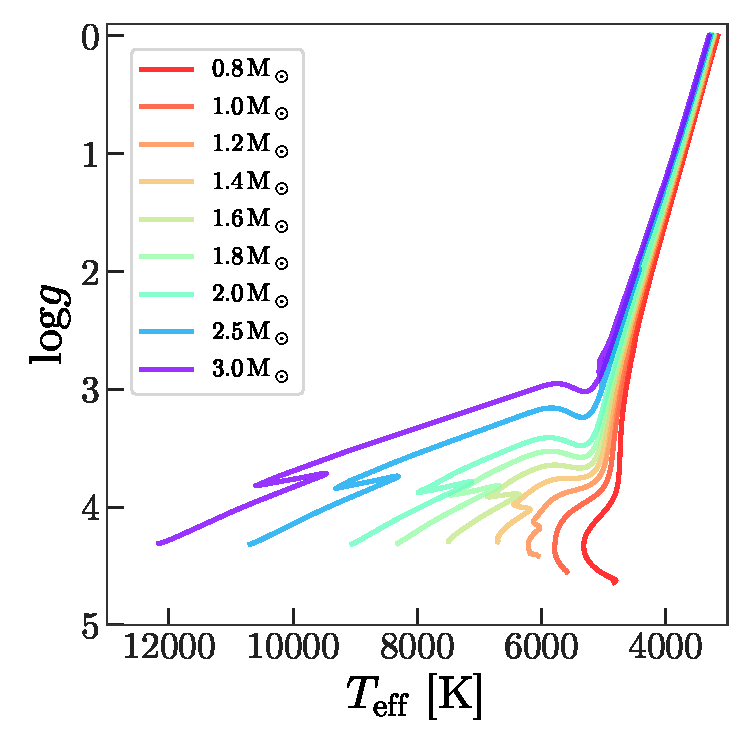
\includegraphics[width=0.6\textwidth]{mesa}
\end{center}
\caption{%
Evolutionary tracks of the eight stellar models we use to simulate the orbital
evolution of a population of binary star systems with an evolved star member.
Horizontal axis shows the effective temperature, $T_\textrm{eff}$, and vertical
axis shows the log-surface-gravity, \logg.
Tracks are colored by the mass of the star.
All models have solar metallicity.
\label{fig:mesa}
}
\end{figure}

We discretize the primary masses generated from the GMMs onto the grid of masses
for which we have \acronym{MESA} models, then use equilibrium tide theory to
compute the change in eccentricity and separation of the companion orbit.
To do this, we solve the coupled differential equations \eqname
s~\ref{eq:dlne}--\ref{eq:dlna} up to the phase of evolution at which the stellar
model has the same (or closest) surface gravity to the simulated primary star.
We use Euler's method with 10,000 time steps between the main sequence and the
given final \logg\ of each primary star, and use linear interpolation to
interpolate the \acronym{MESA} output stellar parameters onto the integration
grid.
We assume that all stars are on their first ascent up the giant branch, which
should underestimate the number of circularized systems with surface gravities
$\logg \sim 2.5$ (i.e. near the red clump, where stars have already reached the
tip of the giant branch).
We assume that the equilibrium tides dominate the circularization process for
all systems and therefore ignore the effect of ``dynamical tides''
(\citealt{who}) during the main sequence phase.
Finally, we assume that all of our systems are detached binaries.

\figurename~\ref{fig:simulated} (middle) shows the final periods and
eccentricities of the simulated systems.
As expected, the circularization period for higher \logg\ systems (i.e. smaller
radii, smaller markers) appears to be close to $\sim 10~\textrm{day}$, but the
circularization period for stars with lower \logg\ (i.e. larger radii, larger
markers) is closer to $\sim 100~\textrm{day}$.
In the right panel we normalize the orbital period by \Psurf:
This rescaling removes the dependence on primary size or \logg and predicts that
circularization should occur around $P / \Psurf \approx 10$.
% except for a few systems that are just reaching the subgiant phase (still have
% high \logg, small markers) apparent in the lower left region of the right panel.

% Notebook: Simulated population
\begin{figure}[htbp]
\begin{center}
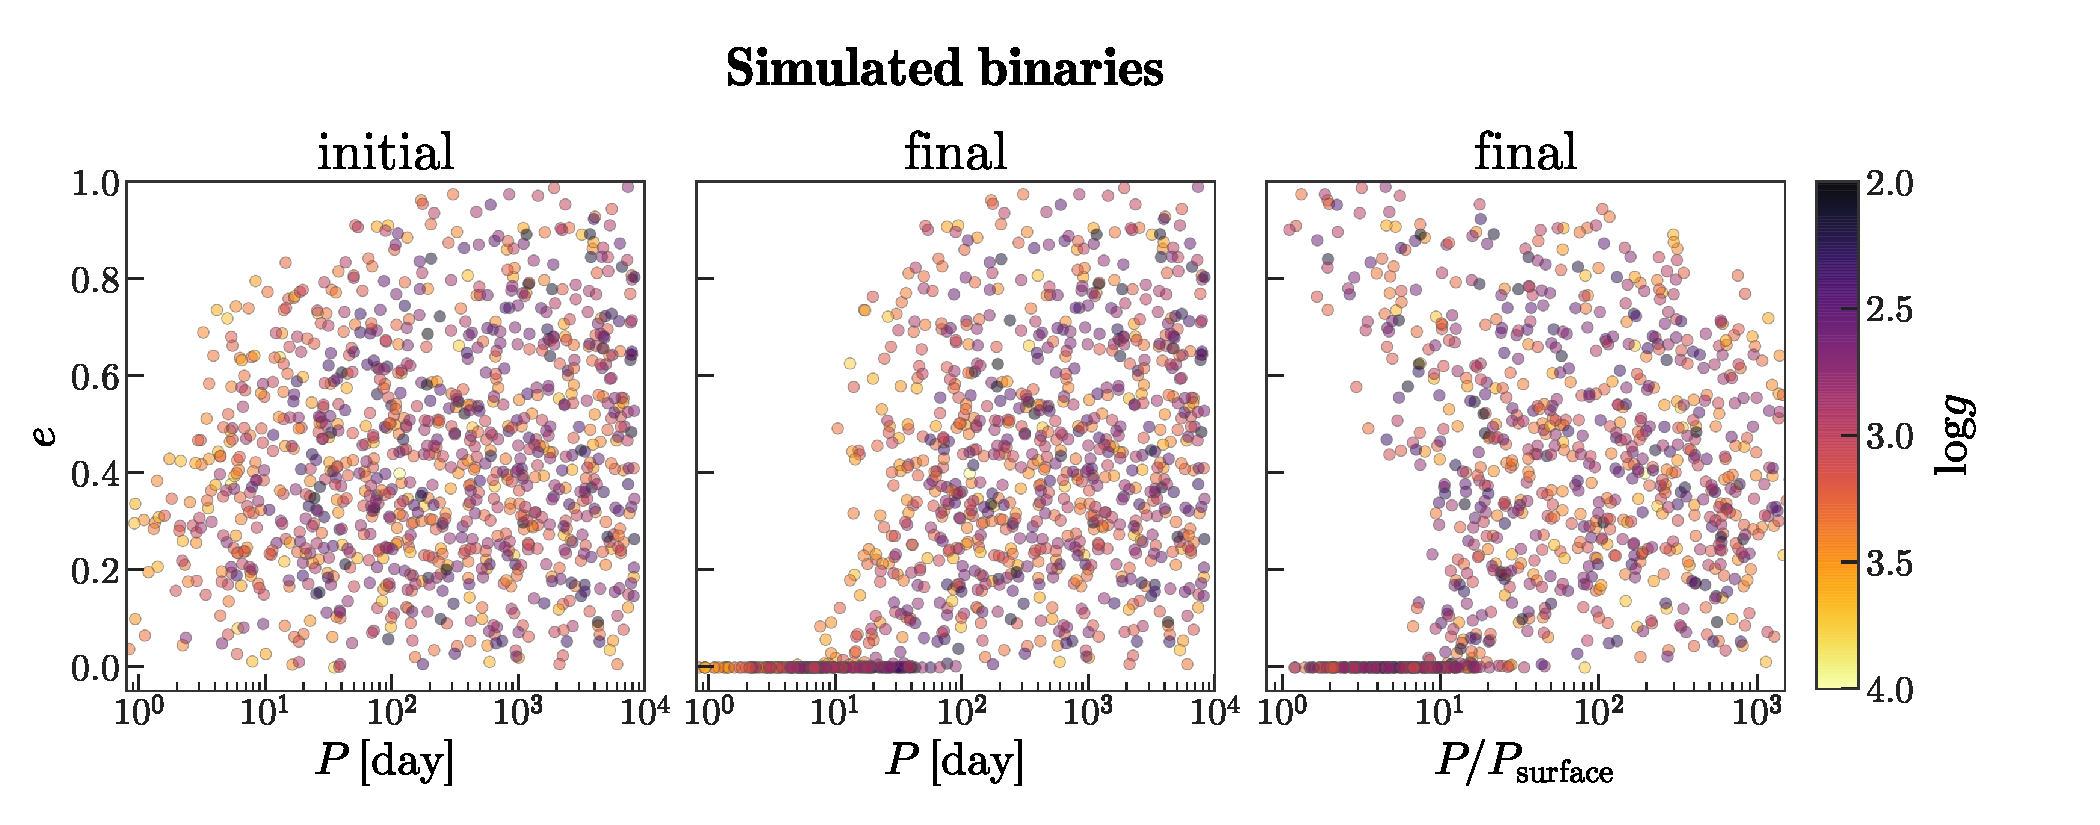
\includegraphics[trim={0 0 1cm 0}, clip, width=\linewidth]{simulated}
\end{center}
\caption{%
Simulated binary star systems with one giant star member.
Points are colored by primary mass, $M_1$, and the size indicates the size of
the star, i.e. the surface gravity $\log g$.
\textit{Left:} Distribution of initial orbital parameters period, $P$, and
eccentricity, $e$.
\textit{Middle:} Final distribution of period and eccentricity after computing
the change in eccentricity from evolution of the primary star.
\textit{Right:} Final distribution of period and eccentricity, with period
normalized by \Psurf, the period of a hypothetical, point-mass
companion whose orbit grazes the surface of the primary star at pericenter.
\label{fig:simulated}
}
\end{figure}


\section{Results}
\label{sec:results}

Our sample of binaries contains primary stars with a range of stellar parameters
(\figurename~\ref{fig:logg-teff-m1}), and therefore a range of expected
circularization periods.
\figurename~\ref{fig:P-e-grid} shows orbital period and eccentricity for all
systems in bins of primary surface gravity:
From top left to bottom right shows bins of decreasing surface gravity, i.e.
from subgiants to giant branch stars.
Vertical dashed lines at $10~\textrm{day}$ and $100~\textrm{day}$ are meant as
reference lines.
Note the steadily increasing circularization period from top left to bottom
right as the typical size of the primary increases.

To compare with predictions from the simulated systems
(\sectionname~\ref{sec:theory}) and to remove the dependence on the size of
the primary, \figurename~\ref{fig:PeK} (left) shows normalized period and
eccentricity for all systems.
We compute \Psurf\ (\eqname~\ref{eq:Psurf}) for all systems by assuming that all
primary stars have masses equal to the median mass over all stars with prior
mass measurements in this sample, $\med{M_1} = 1.36~\msun$, and all companions
have masses equal to the median over minimum companion masses $\med{M_{2,
\textrm{min}}} = 0.5~\msun$.
The sharp transition in eccentricity around $P/\Psurf \approx 10$ apparent in
\figurename~\ref{fig:PeK} (left) appears to be qualitatively consistent with the
prediction from the simulated population visualized in
\figurename~\ref{fig:simulated}.
Right panel of \figurename~\ref{fig:PeK} shows the inferred radial velocity
amplitude of the primary for these same systems.

% Notebook: Results
\begin{figure}[h]
\begin{center}
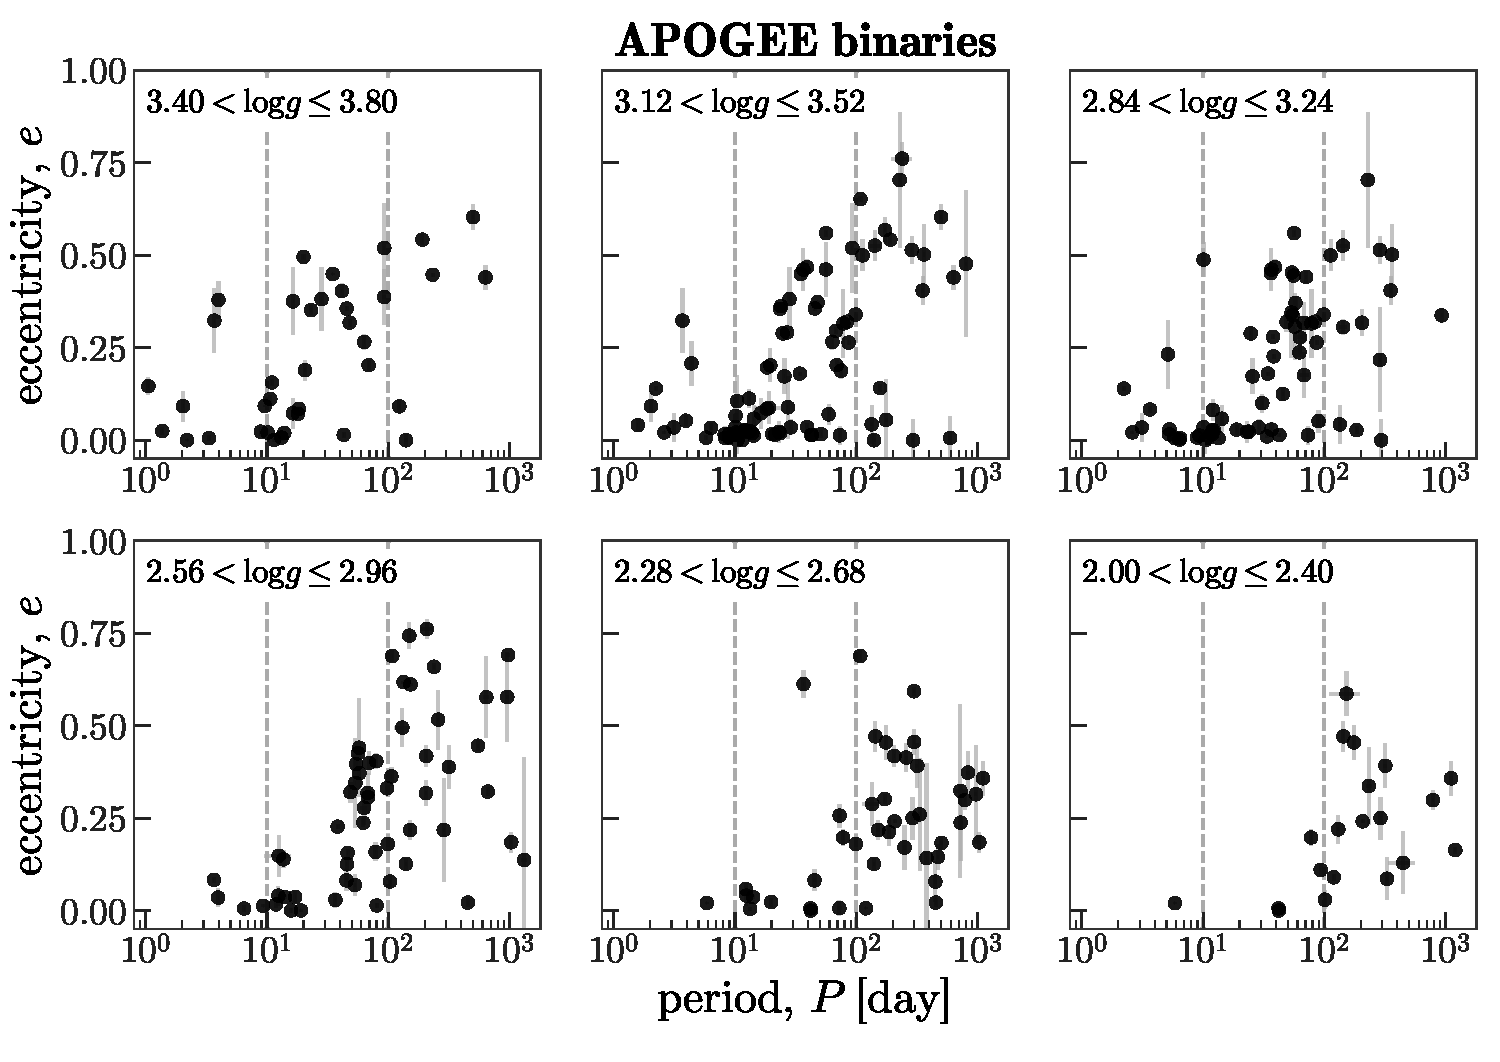
\includegraphics[width=\textwidth]{P-e-grid}
\end{center}
\caption{%
Orbital period and eccentricity for all systems considered in this work.
Each panel shows systems in the specified bin of primary surface gravity, \logg.
Vertical gray lines show periods of $10~\textrm{day}$ and $100~\textrm{day}$:
binaries with subgiant members (top left) show circularization periods close to
$10~\textrm{day}$, whereas binaries with RGB members (bottom right) show
circularization periods close to $100~\textrm{day}$.
Intermediate bins show steadily increasing circularization periods with
decreasing \logg.
\label{fig:P-e-grid}
}
\end{figure}

% Notebook: Results
\begin{figure}[h]
\begin{center}
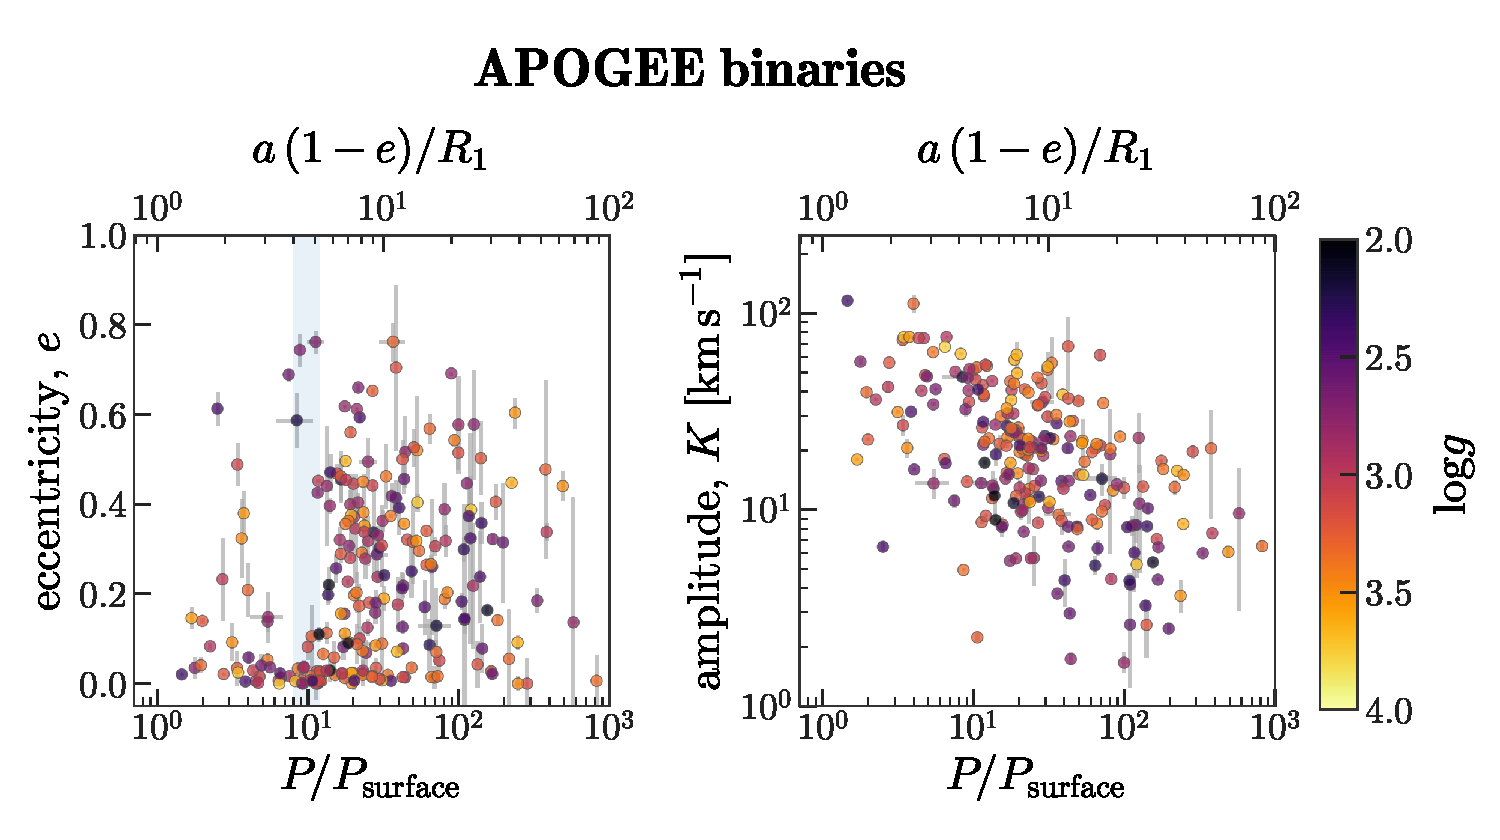
\includegraphics[width=\textwidth]{P-e-K}
\end{center}
\caption{%
\textit{Left panel:} Orbital period and eccentricity for all high-$K$ unimodal
systems with $\log g > 2$, with period values normalized by the orbital period
of a hypothetical companion at the surface of each primary star,
$P_{\textrm{surface}}$, assuming $M_1 = 1.36~\msun$ and $M_2 = 0.5~\msun$.
Stars in the \apogee\ \DR\ red clump catalog are outlined in red.
The sharp transition from eccentric systems to almost all circular orbits at
$P/P_\textrm{surface} \approx 7$ is likely an outcome of tidal circularization.
\textit{Right panel:} Normalized period and inferred radial velocity amplitude
for the same systems.
Points below $P/P_\textrm{surface} = 1$ are likely systems where the primary and
companion mass assumptions used to compute $P_\textrm{surface}$ are invalid.
\label{fig:PeK}
}
\end{figure}

Assuming that the semi-major axes of the \apogee\ binaries have remained
constant, and with assumptions about the primary and companion masses, we can
also compute the expected change in eccentricity, $\Delta \ln e$, for each
binary (see also \figurename~4 in \citealt{Verbunt:1995}).
To compute this quantity for all systems, we assume that the primary mass is
$M_1 = 1.4~\msun$ and the companion mass is $M_2 = 0.5~\msun$, close to the
median values for the systems where these masses are measured.
We use the $1.4~\msun$ \acronym{MESA} model to integrate \eqname~\ref{eq:dlne}
up to the measured \logg\ of the primary star, again using 10,000 time steps,
and linear interpolation to compute the stellar parameters at each time step.

\figurename~\ref{fig:dlne} shows the expected change in eccentricity plotted
against the observed eccentricity for all of the \apogee\ binaries.
With the exception of a few outliers, systems that are predicted to have large
negative changes to the log-eccentricity are circular.
This confirms the conclusions of previous work based on a much smaller sample of
giant star binaries (\citealt{Verbunt:1995}): the theory of equilibrium tides
successfully explains the observed eccentricities of close binaries with
member stars that have large convective envelopes.

\begin{figure}[h]
\begin{center}
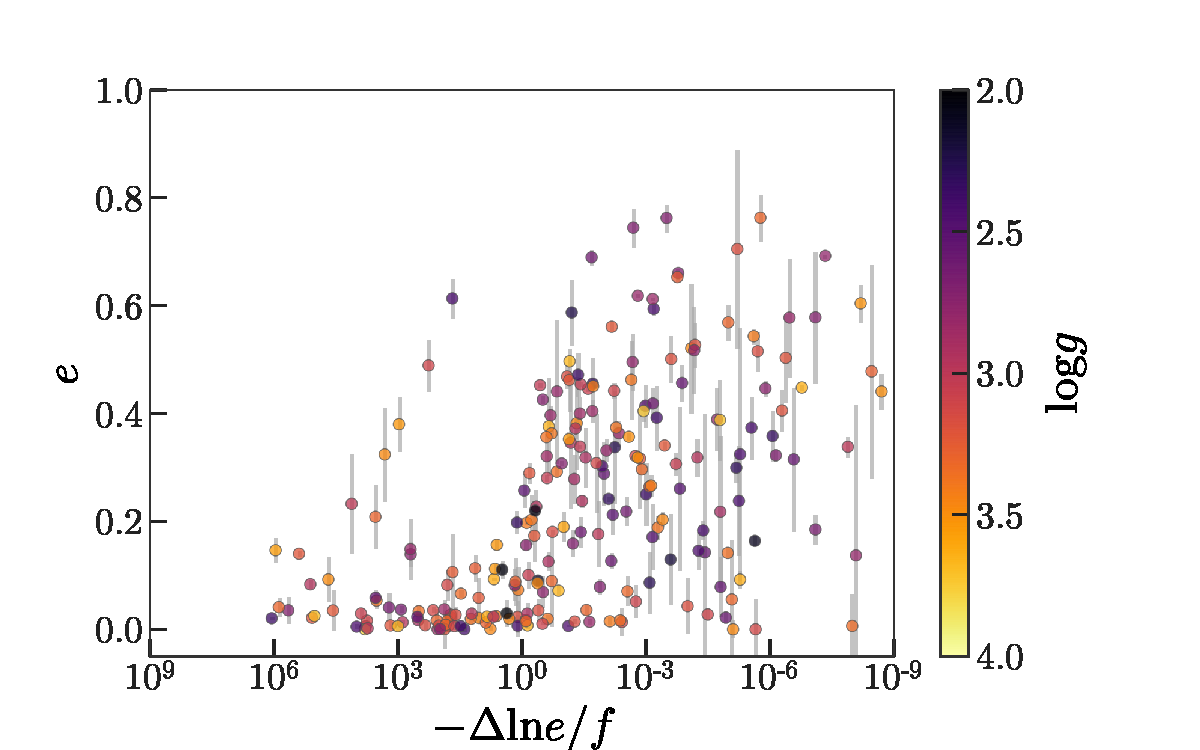
\includegraphics[width=\textwidth]{dlne}
\end{center}
\caption{%
TODO:
\label{fig:dlne}
}
\end{figure}

\section{Discussion} \label{sec:discussion}

- TODO: caveats with the assumptions about primary mass above. Stars have a range of masses, companions. But overall looks good and consistent with VP95!

- Low-ecc "spur" extends to larger periods. This could be: (a) systems where the companion already evolved (even more efficient), (b) systems that started with smaller ecc. to begin with, (c) red clump stars - circularized at TRGB.

- Outliers? Short-period but eccentric systems?

- Incompleteness at high eccentricity: APOGEE sampling


\section{Conclusions}

- Large spectroscopic surveys (SDSS V) can do binary star science

- Gaia RV's end of mission

- Expand to SB2 as well


\acknowledgements

It is a pleasure to thank
Matteo Cantiello (Flatiron),
Jeremy Goodman (Princeton),
David W. Hogg (NYU/Flatiron/MPIA),
Hans-Walter Rix (MPIA),
and Joshua Winn (Princeton).

The authors are pleased to acknowledge that the work reported on in this
paper was substantially performed at the TIGRESS high performance computer
center at Princeton University which is jointly supported by the Princeton
Institute for Computational Science and Engineering and the Princeton
University Office of Information Technology's Research Computing department.

\software{
    \package{Astropy} (\citealt{Astropy-Collaboration:2013}),
    \package{emcee} (\citealt{Foreman-Mackey:2013}),
    \package{IPython} (\citealt{Perez:2007}),
    \package{matplotlib} (\citealt{Hunter:2007}),
    \package{numpy} (\citealt{Van-der-Walt:2011}),
    \package{scikit-learn} (\citealt{Pedregosa:2011}),
    \package{scipy} (\url{https://www.scipy.org/}),
    \package{schwimmbad} (\citealt{Price-Whelan:2017a}),
    \package{sqlalchemy} (\url{https://www.sqlalchemy.org/}),
    \package{thejoker} (\citealt{Price-Whelan:2017b}).
    % \package{twobody} (\todo{twobody zenodo}).
}

\facility{\sdssiv, \apogee}

\clearpage

\bibliographystyle{aasjournal}
\bibliography{refs}


\end{document}
